\chapter{Introduction}
\label{chapter:intro}

In past years, the FLAME project, a collaborative effort between The
University of Texas at Austin and Universidad Jaime I de Castellon, 
developed a unique methodology, notation, and set of APIs for deriving
and representing linear algebra libraries.
In an effort to better promote the techniques characteristic to the FLAME
project, we have implemented a functional prototype library that demonstrates
%featured results and insights from the last decade of research.
findings and insights from the last decade of research.
We call this library {\em libflame}.\footnote{Henceforth, we will typeset
the name of the library in a fixed-width font, just as we typeset the names of
executable programs and scripts.}

The primary purpose of \libflame is to provide the scientific and
numerical computing communities with a modern, high-performance dense linear
algebra library that is extensible, easy to use, and available under an open
source license.
%The primary purpose of \libflame is to provide the scientific and
%numerical computing communities with a modern, high-performance dense linear
%algebra library that is extensible, easy to use, and available under an open
%source license.
%\libflame is a derivative of the broader FLAME project, which was started in
%2000 as a collaborative effort between The University of Texas at Austin and
%Universidad Jaime I de Castellon.
%In that time, the group, which
%previously brought us the FLAME methodology, notation, and APIs for deriving
%and representing linear algebra libraries.
%\libflame is the product of years of research and software development by
%leading members of the FLAME project in the Department of Computer Sciences
%at The University of Texas at Austin.
%While \libflame, as a library, is the product of leading members of the FLAME
%project at The University of Texas at Austin, the broader FLAME project is
%and has always been a collaborative effort between The University of Texas at
%Austin and Universidad Jaime I.
%The implementations present within \libflame were heavily influenced by the ideas
%and insights contributed to the FLAME effort, including the methodology and notation
%that has become characteristic of the FLAME approach to dense linear algebra.
%\footnote{We would be remiss in not
%acknowledging the our collaborators at the Universidad Jaime I of Spain.
%Our colleagues overseas have made numerous and significant contributions
%to the FLAME effort, as the publication record shows.
%While \libflame consists only of code developed at the University of Texas at
%Austin, many of the {\em ideas} cultivated by our joint research would
%eventually influence and shape the implementations present within \libflame.}
Its developers have published numerous papers and working notes
over the last decade documenting the challenges and motivations that led to the
APIs and implementations present within the \libflame library.
Most of these publications listed in Appendix~\ref{appendix:pubs}.
Seasoned users within scientific and numerical computing circles will quickly
recognize the general set of functionality targeted by \libflamens.
In short, in \libflame we wish to provide not only a framework for developing
dense linear algebra solutions, but also a ready-made library that is, by
almost any metric, easier to use and offers competitive (and in many cases
superior) real-world performance when compared to the more traditional LAPACK
and BLAS libraries \cite{LAPACK3,BLAS1,BLAS2,BLAS2,BLAS3}.



\section{What's provided}

\index{\libflame!features}

The FLAME project is excited to offer potential users numerous reasons to
adopt \libflame into their software solutions.

\paragraph{A solution based on fundamental computer science.}
The FLAME project advocates a new approach to developing linear algebra
libraries.
It starts with a more stylized notation for
expressing loop-based linear algebra algorithms~\cite{inverse-siam,FLAME_WoCo,FLAME,TSoPMC}.
This notation closely resembles how matrix algorithms are naturally
illustrated with pictures.
(See Figure \ref{fig:chol-alg} and Figure \ref{fig:flame-lapack-code} (left).) 
The notation facilitates rigorous formal derivation of algorithms~\cite{FLAME,Recipe,TSoPMC}, which guarantees that the resulting algorithms are correct.

\paragraph{Object-based abstractions and API.}
The BLAS, LAPACK, and ScaLAPACK~\cite{ScaLAPACK} projects place
backward compatibility as a high priority, which hinders progress
towards adopting modern software engineering principles such as object
abstraction.  \libflame is built around opaque structures that hide
implementation details of matrices, such as leading dimensions, and
exports object-based programming interfaces to operate upon these
structures~\cite{FLAME:API}.  Likewise, FLAME algorithms are expressed (and coded) in
terms of smaller operations on sub-partitions of the matrix operands.
This abstraction facilitates programming without array or loop
indices, which allows the user to avoid painful index-related
programming errors altogether.  Figure \ref{fig:flame-lapack-code}
compares the coding styles of \libflame and LAPACK, highlighting the
inherent elegance of FLAME code and its striking resemblance to the
corresponding FLAME algorithm shown in Figure \ref{fig:chol-alg}.
This similarity is quite intentional, as it preserves the clarity of
the original algorithm as it would be illustrated on a white-board or
in a publication.


\resetsteps      % Reset all the commands to create a blank worksheet  

% Define the operation to be computed

%\renewcommand{\operation}{ \left[ A \right] := \mbox{\sc FLA_Chol_l\_blk}( A ) }
\renewcommand{\routinename}{ A \becomes \mbox{\sc Chol\_l\_blk\_var2( A ) } }

% Step 1a: Precondition 

\renewcommand{\precondition}{
  A = \hat{A}
}

% Step 1b: Postcondition 

\renewcommand{\postcondition}{ 
  \left[A \right]
  =
  \mbox{FLA_Chol_l}( A )
}

% Step 2: Invariant 
% Note: Right-hand side of equalities must be updated appropriately

\renewcommand{\invariant}{
  \FlaTwoByTwo{A_{TL}}{A_{TR}}
              {A_{BL}}{A_{BR}} =
  \FlaTwoByTwo{\hat{A}_{TL}}{\hat{A}_{TR}}
              {\hat{A}_{BL}}{\hat{A}_{BR}}
}

% Step 3: Loop-guard 

\renewcommand{\guard}{
  m( A_{TL} ) < m( A )
}

% Step 4: Initialize 

\renewcommand{\partitionings}{
  $
  A \rightarrow
  \FlaTwoByTwo{A_{TL}}{A_{TR}}
              {A_{BL}}{A_{BR}}
  $
}

\renewcommand{\partitionsizes}{
$ A_{TL} $ is $ 0 \times 0 $
}

% Step 5a: Repartition the operands 

\renewcommand{\blocksizeftex}{b}

\renewcommand{\repartitionings}{
$
  \FlaTwoByTwo{A_{TL}}{A_{TR}}
              {A_{BL}}{A_{BR}}
  \rightarrow
  \FlaThreeByThreeBR{A_{00}}{A_{01}}{A_{02}}
                    {A_{10}}{A_{11}}{A_{12}}
                    {A_{20}}{A_{21}}{A_{22}}
$
}

\renewcommand{\repartitionsizes}{
  $ A_{11} $ is $ b \times b $
}

% Step 5b: Move the double lines 

\renewcommand{\moveboundaries}{
$
  \FlaTwoByTwo{A_{TL}}{A_{TR}}
              {A_{BL}}{A_{BR}}
  \leftarrow
  \FlaThreeByThreeTL{A_{00}}{A_{01}}{A_{02}}
                    {A_{10}}{A_{11}}{A_{12}}
                    {A_{20}}{A_{21}}{A_{22}}
$
}

% Step 6: State after repartitioning
% Note: The below needs editing!!!

\renewcommand{\beforeupdate}{
  \FlaThreeByThreeBR{A_{00}}{A_{01}}{A_{02}}
                    {A_{10}}{A_{11}}{A_{12}}
                    {A_{20}}{A_{21}}{A_{22}}
=
  \FlaThreeByThreeBR{\hat{A}_{00}}{\hat{A}_{01}}{\hat{A}_{02}}
                    {\hat{A}_{10}}{\hat{A}_{11}}{\hat{A}_{12}}
                    {\hat{A}_{20}}{\hat{A}_{21}}{\hat{A}_{22}}
}

% Step 7: State after moving of double lines
% Note: The below needs editing!!!

\renewcommand{\afterupdate}{
  \FlaThreeByThreeTL{A_{00}}{A_{01}}{A_{02}}
                    {A_{10}}{A_{11}}{A_{12}}
                    {A_{20}}{A_{21}}{A_{22}}
=
  \FlaThreeByThreeTL{\hat{A}_{00}}{\hat{A}_{01}}{\hat{A}_{02}}
                    {\hat{A}_{10}}{\hat{A}_{11}}{\hat{A}_{12}}
                    {\hat{A}_{20}}{\hat{A}_{21}}{\hat{A}_{22}}
}

% Step 8: Insert the updates required to change the 
%         state from that given in Step 6 to that given in Step 7
% Note: The below needs editing!!!

\renewcommand{\update}{
$
  \begin{array}{ll}
                                             & \\[-2.5mm]
    A_{11} \becomes A_{11} - A_{10} A_{11}^T & \hspace{0.55in} \mbox{\sc (syrk)} \\[0.5mm]
    A_{21} \becomes A_{21} - A_{20} A_{10}^T & \hspace{0.55in} \mbox{\sc (gemm)} \\[0.5mm]
    A_{11} \becomes \Chol{A_{11}}            &                                   \\[0.1mm]
    A_{21} \becomes A_{21} A_{11}^{-T}       & \hspace{0.55in} \mbox{\sc (trsm)}
  \end{array}
$
}



\begin{figure}[tbp]
\begin{center}
\footnotesize\FlaAlgorithm
\end{center}
\caption{
Blocked Cholesky factorization (variant 2) expressed as a FLAME algorithm.
Subproblems annotated as {\sc syrk}, {\sc gemm}, and {\sc trsm} correspond
to Level-3 BLAS operations.
}
\label{fig:chol-alg}
\end{figure}


\begin{figure}[tbp]
\begin{center}
\begin{tabular}{|c|c|}
\hline
% --------------------------------------
libflame & LAPACK \\ \hline
% --------------------------------------
% & \\
% --------------------------------------
\begin{minipage}[t]{3in}
{\tiny
\begin{verbatim}
FLA_Error FLA_Chol_l_blk_var2( FLA_Obj A, dim_t nb_alg )
{
  FLA_Obj ATL,   ATR,      A00, A01, A02,
          ABL,   ABR,      A10, A11, A12,
                           A20, A21, A22;
  dim_t b;
  int value;

  FLA_Part_2x2( A,    &ATL, &ATR,
                      &ABL, &ABR,     0, 0, FLA_TL );

  while ( FLA_Obj_length( ATL ) < FLA_Obj_length( A ) )
  {
    b = min( FLA_Obj_length( ABR ), nb_alg );

    FLA_Repart_2x2_to_3x3( ATL, /**/ ATR,       &A00, /**/ &A01, &A02,
                        /* ************* */   /* ******************** */
                                                &A10, /**/ &A11, &A12,
                           ABL, /**/ ABR,       &A20, /**/ &A21, &A22,
                           b, b, FLA_BR );

    /* ---------------------------------------------------------------- */

    FLA_Syrk( FLA_LOWER_TRIANGULAR, FLA_NO_TRANSPOSE, 
              FLA_MINUS_ONE, A10, FLA_ONE, A11 );

    FLA_Gemm( FLA_NO_TRANSPOSE, FLA_TRANSPOSE, 
              FLA_MINUS_ONE, A20, A10, FLA_ONE, A21 );

    value = FLA_Chol_unb_external( FLA_LOWER_TRIANGULAR, A11 );

    if ( value != FLA_SUCCESS )
      return ( FLA_Obj_length( A00 ) + value );

    FLA_Trsm( FLA_RIGHT, FLA_LOWER_TRIANGULAR, 
              FLA_TRANSPOSE, FLA_NONUNIT_DIAG, 
              FLA_ONE, A11, A21 );

    /* ---------------------------------------------------------------- */

    FLA_Cont_with_3x3_to_2x2( &ATL, /**/ &ATR,       A00, A01, /**/ A02,
                                                     A10, A11, /**/ A12,
                            /* ************** */  /* ****************** */
                              &ABL, /**/ &ABR,       A20, A21, /**/ A22,
                              FLA_TL );
  }

  return value;
}
\end{verbatim}
}
\end{minipage}
&
\begin{minipage}[t]{3in}
{\tt \tiny
\begin{verbatim}
      SUBROUTINE DPOTRF( UPLO, N, A, LDA, INFO )

      CHARACTER          UPLO
      INTEGER            INFO, LDA, N
      DOUBLE PRECISION   A( LDA, * )

      DOUBLE PRECISION   ONE
      PARAMETER          ( ONE = 1.0D+0 )
      LOGICAL            UPPER
      INTEGER            J, JB, NB
      LOGICAL            LSAME
      INTEGER            ILAENV
      EXTERNAL           LSAME, ILAENV
      EXTERNAL           DGEMM, DPOTF2, DSYRK, DTRSM, XERBLA
      INTRINSIC          MAX, MIN

      INFO = 0
      UPPER = LSAME( UPLO, 'U' )
      IF( .NOT.UPPER .AND. .NOT.LSAME( UPLO, 'L' ) ) THEN
         INFO = -1
      ELSE IF( N.LT.0 ) THEN
         INFO = -2
      ELSE IF( LDA.LT.MAX( 1, N ) ) THEN
         INFO = -4
      END IF
      IF( INFO.NE.0 ) THEN
         CALL XERBLA( 'DPOTRF', -INFO )
         RETURN
      END IF

      INFO = 0
      UPPER = LSAME( UPLO, 'U' )

      IF( N.EQ.0 )
     $   RETURN

      NB = ILAENV( 1, 'DPOTRF', UPLO, N, -1, -1, -1 )
      IF( NB.LE.1 .OR. NB.GE.N ) THEN
         CALL DPOTF2( UPLO, N, A, LDA, INFO )
      ELSE
         IF( UPPER ) THEN    
*********** Upper triangular case omited for purposes of fair comparison.
         ELSE
            DO 20 J = 1, N, NB
               JB = MIN( NB, N-J+1 )
               CALL DSYRK( 'Lower', 'No transpose', JB, J-1, -ONE,
     $                     A( J, 1 ), LDA, ONE, A( J, J ), LDA )
               CALL DPOTF2( 'Lower', JB, A( J, J ), LDA, INFO )
               IF( INFO.NE.0 )
     $            GO TO 30
               IF( J+JB.LE.N ) THEN
                  CALL DGEMM( 'No transpose', 'Transpose', N-J-JB+1, JB,
     $                        J-1, -ONE, A( J+JB, 1 ), LDA, A( J, 1 ),
     $                        LDA, ONE, A( J+JB, J ), LDA )
                  CALL DTRSM( 'Right', 'Lower', 'Transpose', 'Non-unit',
     $                        N-J-JB+1, JB, ONE, A( J, J ), LDA,
     $                        A( J+JB, J ), LDA )
               END IF
   20       CONTINUE
         END IF
      END IF
      GO TO 40
   30 CONTINUE
      INFO = INFO + J - 1
   40 CONTINUE
      RETURN
      END
\end{verbatim}
}
\end{minipage}
\\
% --------------------------------------
 & \\ \hline
% --------------------------------------
\end{tabular}
\end{center}
\caption{
%The algorithm shown in Figure \ref{fig:chol-alg} implemented with
%FLAME/C code (left), representing the
%style of coding found in libflame, and Fortran-77 code (right)
%obtained from LAPACK. 
The algorithm shown in Figure \ref{fig:chol-alg} implemented with
FLAME/C code (left) and Fortran-77 code (right).
The FLAME/C code represents the style of coding found in libflame
while the Fortran-77 code was obtained from LAPACK.
}
\label{fig:flame-lapack-code}
\end{figure}


\begin{figure}[tbp]
\begin{center}
%\begin{tabular}{c}

%\epsfig{figure=pics/chol_l_itanium2.eps, width=4.00in}
%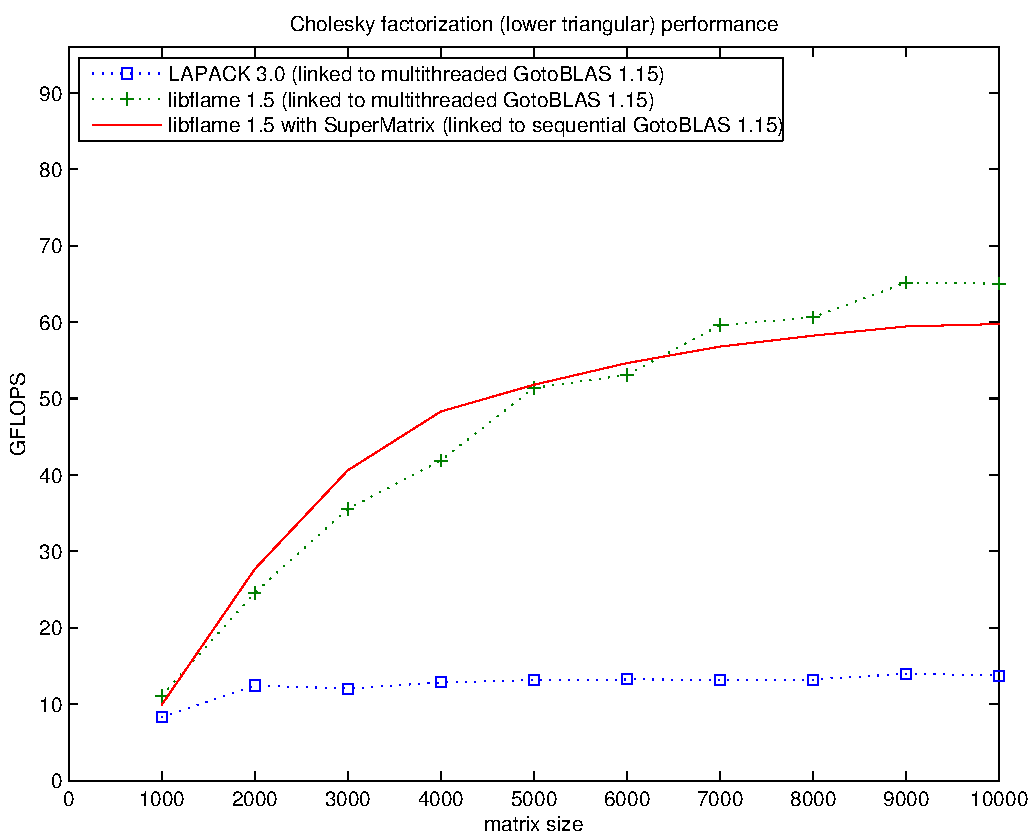
\includegraphics[width=6.5in]{pics/chol_l_itanium2-embedded.pdf}
%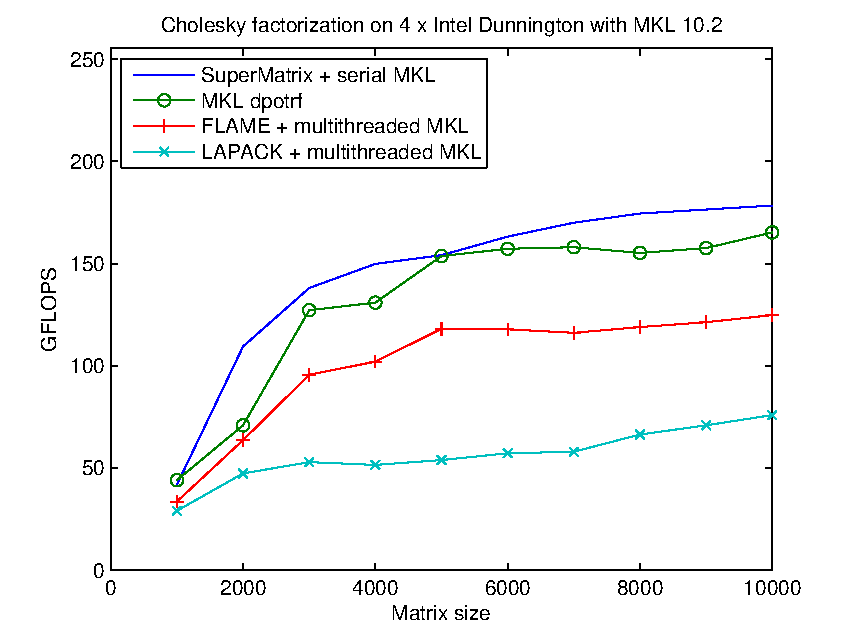
\includegraphics[width=6.5in]{pics/chol_l_dunnington.pdf}
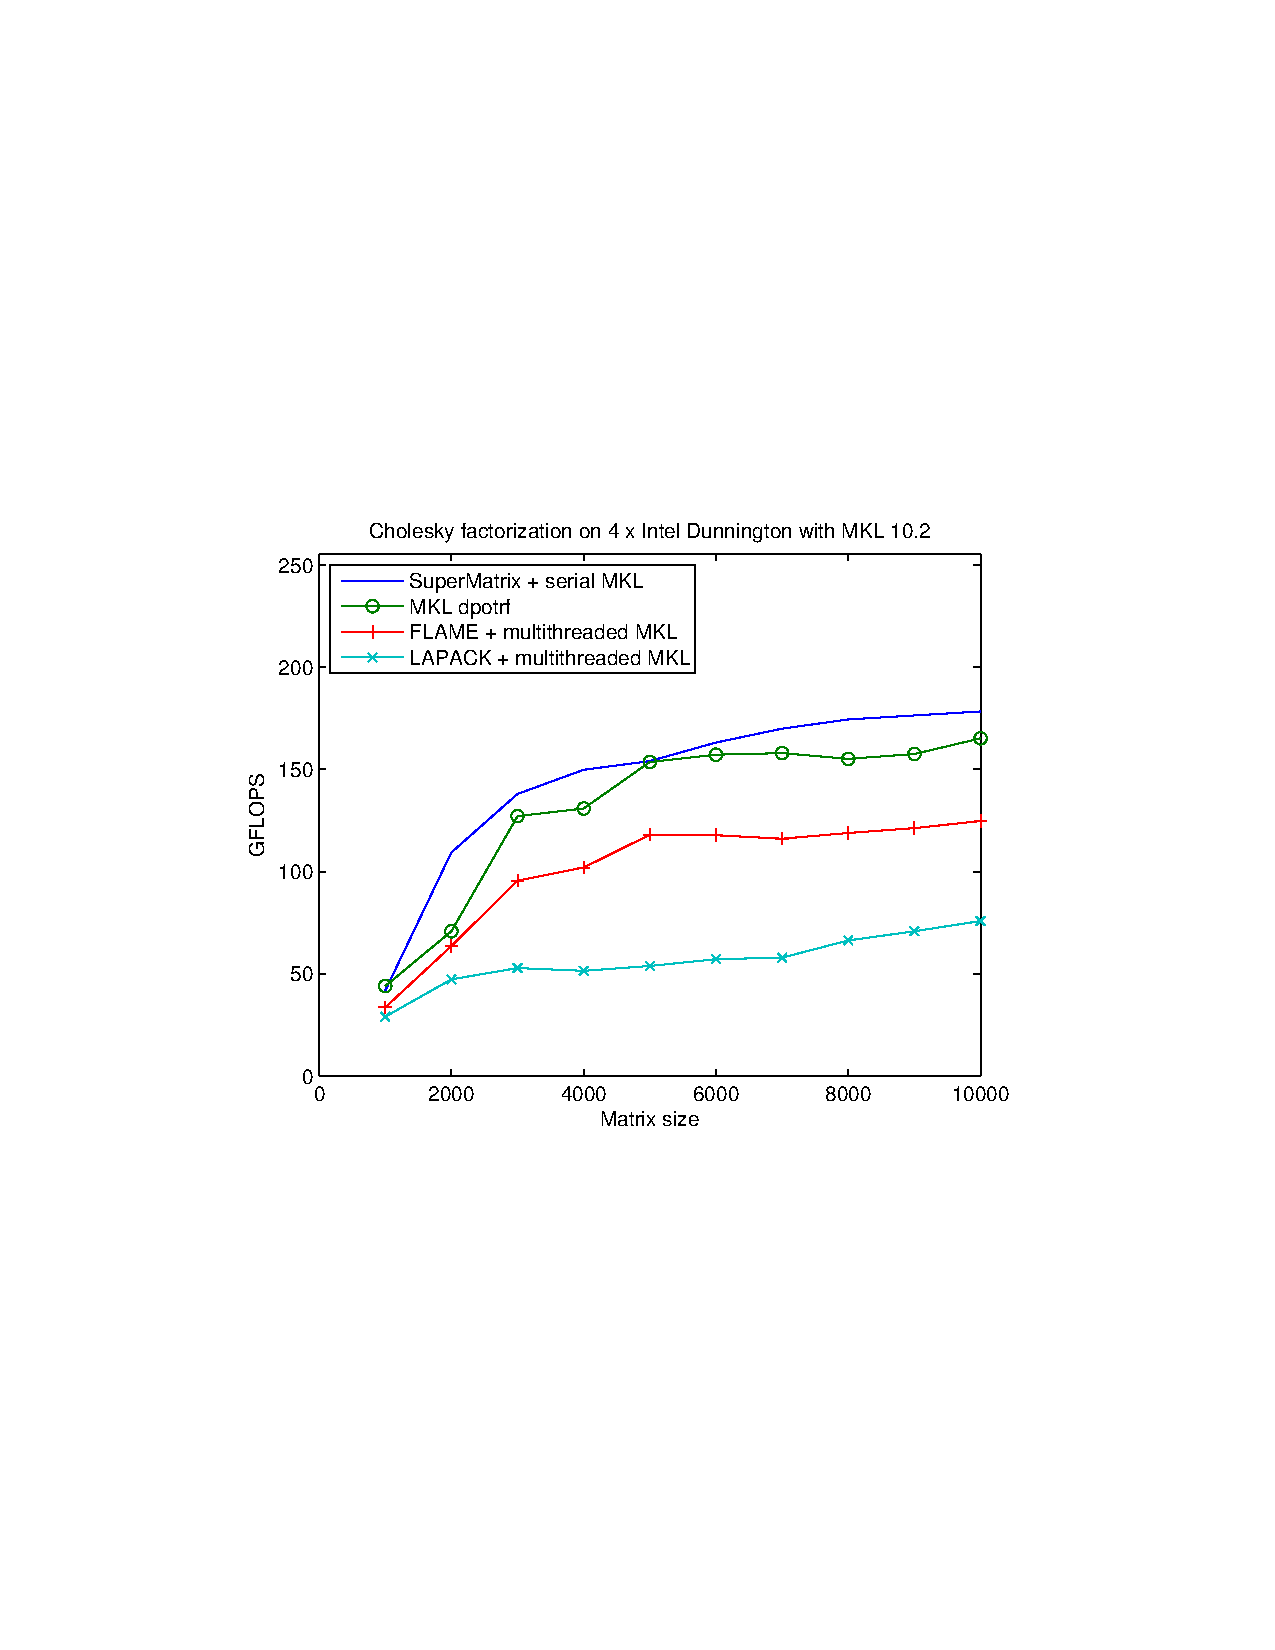
\includegraphics[width=6.5in]{pics/chol_l_dunnington-embedded.pdf}

%\end{tabular}
\end{center}
\caption{
Performance of Cholesky factorization implementations measured on a
24 core Intel ``Dunnington'' system.
Theoretical peak system performance is 255 GFLOPS.
libflame uses variant 3 while LAPACK uses variant 2.
For non-SuperMatrix experiments, MKL was invoked in multithreaded
mode.
For SuperMatrix experiments, MKL parallelism was disabled.
Blocksizes were tuned individually for each problem size tested.
}
\label{fig:chol-perf}
\end{figure}


\paragraph{Educational value.}
Aside from the potential to introduce students to formal algorithm
derivation, FLAME serves as an excellent vehicle for teaching linear
algebra algorithms in a classroom setting.
The clean abstractions afforded by the API also make FLAME ideally suited
for instruction of high-performance linear algebra courses at the
undergraduate and graduate level.
Robert van de Geijn routinely uses FLAME in his linear algebra and
numerical analysis courses.
%%% Some colleagues of the FLAME project are even beginning to use the
%%% notation to teach classes elsewhere around the country, including
%%% Tim Mattson of Intel Corporation.
Historically, the BLAS/LAPACK style of coding has been used in these
pedagocal settings.  However, we believe that coding in that manner
obscures the algorithms; students often get bogged down debugging the
frustrating errors that often result from indexing directly into
arrays that represent the matrices.

\paragraph{A complete dense linear algebra framework.}
Like LAPACK, \libflame provides ready-made implementations of common
linear algebra operations.  The implementations found in \libflame
mirror many of those found in the BLAS and LAPACK packages.  However,
\libflame differs from LAPACK in two important ways: First, it
provides families of algorithms for each operation so that the best
can be chosen for a given circumstance~\cite{Bientinesi:2008:FAR}.  Second, it
provides a framework for building complete custom linear algebra
codes.  We believe this makes it a more useful environment as it
allows the user to quickly chose and/or prototype a linear algebra
solution to fit the needs of the application.

\paragraph{High performance.}
In our publications and performance graphs, we do our best to dispel the
myth that user- and programmer-friendly linear algebra codes cannot yield
high performance.
Our FLAME implementations of operations such as Cholesky factorization and
triangular matrix inversion often outperform the corresponding implementations
currently available in LAPACK~\cite{Bientinesi:2008:FAR}.
Figure \ref{fig:chol-perf} shows an example of the performance increase
made possible by using \libflame for a Cholesky factorization, when compared
to LAPACK.
Many instances of the \libflame performance advantage result from the fact
that LAPACK provides only one variant (algorithm) of most operations,
while \libflame provides many variants.
This allows the user and/or library developer to choose which algorithmic
variant is most appropriate for a given situation.
Currently, \libflame relies only on the presence of a core set of highly
optimized unblocked routines to perform the small sub-problems found in FLAME
algorithm codes.
%
%For future use:
%Additional performance results may be found at our linear algebra
%wiki. 

\paragraph{Dependency-aware multithreaded parallelism.}
Until recently, the most common method of getting shared-memory parallelism
from LAPACK routines by simply linking to multithreaded BLAS.
This low-level solution requires no changes to LAPACK code but also suffers
from sharp limitations in terms of efficiency and scalability for small-
and medium-sized matrix problems.
The fundamental bottleneck to introducing parallelism directly within many
algorithms is the web of data dependencies that inevitably exists between
sub-problems.
The \libflame project has developed a runtime system, SuperMatrix, to detect
and analyze dependencies found within FLAME algorithms-by-blocks
(algorithms whose sub-problems operate only on block operands)%
~\cite{spaa2007,SuperMatrix:PPoPP08,SuperMatrix:PPoPP09,SuperMatrix:TOMS}.
Once dependencies are known, the system schedules sub-operations to
independent threads of execution.
This system is completely abstracted from the algorithm that is being
parallelized and requires virtually no change to the algorithm code, but at
the same time exposes abundant high-level parallelism.
We have observed that this method provides increased performance for a
range of small- and medium-sized problems, as shown in Figure
\ref{fig:chol-perf}.
The most recent version of LAPACK does not offer any similar
mechanism.\footnote{Some of the lead developers of LAPACK have independently
investigated these ideas as part of a spin-off project,
PLASMA \cite{LAWN190,LAWN191,emmanuel2009}.}

\paragraph{Support for hierarchical storage-by-blocks.}
Storing matrices by blocks, a concept advocated years ago by Fred Gustavson
of IBM, often yields performance gains through improved spatial locality~\cite{gustavson1,SIAMrec,gustavson3}.
Instead of representing matrices as a single linear array of data with a
prescribed leading dimension as legacy libraries require (for column- or
row-major order), the storage scheme is encoded into the matrix object.
Here, internal elements refer recursively to child objects that
represent sub-matrices.
Currently, \libflame provides a subset of the conventional API that supports
hierarchical matrices, allowing users to create and manage such matrix
objects as well as convert between storage-by-blocks and conventional
``flat'' storage schemes \cite{SuperMatrix:TOMS,FLASH:TR}. 

\paragraph{Advanced build system.}
From its early revisions, \libflame distributions have been bundled with a
robust build system, featuring automatic makefile creation and a
configuration script conforming to GNU standards (allowing the user to run
the {\tt ./configure; make; make install} sequence common to many open source
software projects).
Without any user input, the configure script searches for and chooses
compilers based on a pre-defined preference order for each architecture.
The user may request specific compilers via the configure interface, or
enable other non-default features of \libflame such as custom memory
alignment, multithreading (via POSIX threads or OpenMP), compiler options
(debugging symbols, warnings, optimizations), and memory leak detection.
The reference BLAS and LAPACK libraries provide no configuration support
and require the user to manually modify a makefile with appropriate
references to compilers and compiler options depending on the host
architecture. 

\paragraph{Windows support.}
While \libflame was originally developed for GNU/Linux and UNIX environments,
we have in the course of its development had the opportunity to port the
library to Microsoft Windows.
The Windows port features a separate build system implemented with Python
and \nmakens, the Microsoft analogue to the \make utility found in UNIX-like
environments.
As of this writing, the port is still relatively new and therefore should be
considered experimental.
However, we feel \libflame for Windows is useable for many in our audience.
We invite interested users to try the software and, of course, we welcome
feedback to help improve our Windows support, and \libflame in general.

\paragraph{Independence from Fortran and LAPACK.}
The \libflame development team is pleased to offer a high-performance linear
algebra solution that is 100\% Fortran-free.
\libflame is a C-only implementation and does not depend on any external
Fortran libraries such as LAPACK.\footnote{In fact, besides the BLAS
and the standard C libraries, \libflame does not have any external
dependencies---not even {\tt f2c}.}
That said, we happily provide an optional backward compatibility layer,
\lapacktflamens, that maps LAPACK routine invocations to their
corresponding native C implementations in \libflamens.
This allows legacy applications to start taking advantage of \libflame
with virtually no changes to their source code.
Furthermore, we understand that some users wish to leverage highly-optimized
implementations that conform to the LAPACK interface, such as Intel's Math
Kernel Library (MKL).
As such, we allow those users to configure \libflame such that their external
LAPACK implementation is called for the small, performance-senstive unblocked
subproblems that arise within \libflamens's blocked algorithms and
algorithms-by-blocks.




\section{What's not provided}

While we feel that \libflame is a powerful and effective tool, it is not for
everyone.
In this section we list reasons you may want to avoid using \libflamens.

\paragraph{Distributed memory parallelism.}
\libflame does not currently offer distributed memory parallelism.
Some of the FLAME project members once maintained a library called
PLAPACK \cite{PLAPACK_SC97,PLAPACK}, which provided a framework for
implementing dense linear algebra operations in a parallel distributed
memory environment.  However, this library is no longer supported by
the FLAME group.  We have begun preliminary work on rewriting PLAPACK
to incorporate many of the things we've learned while developing the
FLAME methodology.  But until we can finish this rewrite of PLAPACK,
\libflame will not support parallel distributed memory computing.

\paragraph{Out-of-core computation.}
\libflame does not currently support out-of-core computation.
However, the FLAME group has published research based on results from a
prototype extension to \libflame \cite{OOCLU:Para04}.
While this prototype extension is not distributed with \libflamens,
we believe that FLASH with its the hierarchical storage format will
provide us with a relatively straightforward path to incorporating
out-of-core functionality in the future.
Our colleages at Universidad Jaime I de Castellon, however, have more
recent expertise in this area.
Those interested in out-of-core functionality should contact them
directly.

\paragraph{Sparse matrix functionality.}
Algorithms implementated in \libflame do not take advantage of sparseness
that may be present within a matrix, nor does it take advantage of any
special structure beyond the traditional dense matrix forms (triangular,
symmetric, Hermitian), nor does it support special storage formats that
avoid storing the zero elements present in sparse matrices.
Users looking to operate with sparse matrices, especially those that are
large, should look into more specialized software packages that leverage
the properties inherent to your application.

\paragraph{Banded matrix support}
Many routines within the BLAS and LAPACK are specially written to take
advantage of banded matrices.
As with sparse matrices, these routines expect that the matrix arguments
be stored according to a special storage scheme that takes advantage of
the sparsity of the matrix.
Unfortunately, \libflame does not offer any storage scheme targeting banded
matrices, and thus does not include any routines that leverage such storage
within the computation.
Though, our colleages in Spain have reported on work using banded matrices
in algorithms-by-blocks~\cite{SuperMatrix:HPCCS}.

\paragraph{Traditional coding style.}
We are quite proud of \libflame and its interfaces, which we believe are
much easier to use than those of the BLAS and LAPACK.
However, it's entirely possible that switching to the \libflame API is
not feasible for you or your organization.
For example, if you are a Fortran programmer, you may not have the patience
or the liberty to write and use C wrappers to the \libflame routines.
Or, your project may need to remain written in Fortran for reasons beyond
your control.
Whatever the case, we understand and appreciate that coding style imposed
by \libflame may be too different for some users and applications.

\paragraph{Interactive/Interpreted programming}
Some people require a degree of interactivity in their scientific computing
environment.
Good examples of linear algebra tools that supports interpreted programming
are The MathWorks' {\sc matlab} and National Instruments' LabVIEW MathScript.
Programming with {\sc matlab} or LabVIEW MathScript is a great way to prototype
new ideas and flesh out your algorithms before moving them to a high-performance
environment.
While \libflame provides many features and benefits, an interpreted programming
environment is not one of them.
If you require this feature, we encourage you to look at {\sc matlab} as well
as other free alternatives, such as Octave and Sage.

\paragraph{Licensing conflict.}
\libflame is provided as free software to the general public under the
GNU Lesser General Public License, version 2.1,
given in Appendix~\ref{appendix:license}.
However, some organizations prohibit their employees from using (or even
looking at) code that is released under GNU licenses.
If this applies to you, then you should look for software that is
either freely-available\footnote{Some relevant software packages are
considered to be public domain, while others are released under a BSD-like
license.
Some may even be public domain with regard to only certain components.
To err on the side of safety, in cases where the license is not clear, we
refer to these packages collectively as ``freely-available'', particularly
when the authors choose to use this terminology.
Please refer to the homepages of each software package for precise
licensing information.}, or released under a license which is less
restrictive than the LGPL. \\

Whatever the reason, we acknowledge that it may not be practical or even
possible to incorporate \libflame into your software solution.
We hope \libflame fits your needs, but if it does not then we would like to
refer you to other software packages that you may want to consider:
\begin{itemize}
\item {\bf BLAS.}
The official reference implementation of the BLAS is available through the
{\tt netlib} software repository \cite{netlibblas2008}.
It implements basic matrix-matrix operations such as general matrix multiply
as well as several less computationally intensive operations involving one
or more vector operands.
The BLAS is freely-available software.
\item {\bf LAPACK.}
Like the BLAS, the official reference implementation of LAPACK is available
through the netlib software repository \cite{netliblapack2008}.
This library implements many more sophisticated dense linear algebra
operations, such as factorizations, linear system solvers, and eigensolvers.
LAPACK is freely-available software.
\item {\bf ScaLAPACK.}
ScaLAPACK was designed by the creators of the BLAS and LAPACK libraries to
implement dense linear algebra operations for parallel distributed memory
environments.
Its API is similar to that of LAPACK and targets mostly Fortran-77
applications,though it may also be accessed from programs written in C.
ScaLAPACK is freely available software and available through the netlib
software repository \cite{netlibscalapack2008}.
\item {\bf PETSc.}
PETSc, written and maintained by The University of Chicago, provides
parallel solvers for PDEs, and other related tools, with bindings for C,
C++, Fortran, and Python \cite{petsc2008}.
PETSc is available from the University of Chicago under a custom GNU-like
license.
\item {\bf MATLAB.}
The MathWorks' flagship product, {\sc matlab}, is a scientific and numerical
programming environment featuring a rich library of linear algebra, signal
processing, and visualization functions \cite{mathworks2008}.
{\sc matlab} is licensed as a commerical product.
\item {\bf LabVIEW.}
National Instruments offers a commercial solution, LabVIEW MathScript, which
is a component of LabVIEW, that provides an interactive programming environment
compatible with {\sc matlab} \cite{ni2008}.
\item {\bf Octave.}
GNU Octave is a free alternative to {\sc matlab}, providing high-level
interpreted language functionality for scientific and numerical applications.
GNU Octave is distributed under the GNU General Public
License \cite{octave2008}.
\item {\bf Sage.}
Sage, like Octave, is free software that provides much of the functionality
of {\sc matlab}, but also targets users of Magma, Maple, and Mathematica.
Sage is distributed under the GNU General Public License \cite{sage2008}.
\end{itemize}
We thank you for your interest in \libflame and the FLAME project.



\section{Acknowledgments}

The \libflame library was made possible thanks to innovative contributions from
some of the top researchers in the field of dense linear algebra, including
many active members of the FLAME project.
I am flattered and grateful that, despite the fact that the library represents
the hard work of all of these individuals, my colleagues encouraged me to
publish this document without them as coauthors.
Their contributions are well-documented in the many journal papers, conference
proceedings, and working notes published over the last decade.
Citations for many of these publications may be found in Appendix \ref{appendix:pubs}.

Over the years, the FLAME project and the \libflame library effort have been
generously funded by the National Science Foundation grants CCF-0702714,
CCF-0540926, CCF-0342369, ACI-0305163, and ACI-0203685.
In addition, Microsoft, NEC Systems (America), Inc., and National Instruments
have provided significant support.
An equipment donation from Hewlett-Packard has also been invaluable.

{\em Any opinions, findings and conclusions or recommendations expressed in this
material are those of the author(s) and do not necessarily reflect the views of
the National Science Foundation (NSF).}


